\chapter{Introduction}\label{chap:intro}

Pedestrian simulations allow us to ask questions about a place before it is built or altered. Will the food court have enough tables during the lunch rush, will two shifts of office workers compete for the same desks, and will one of the exits become a choke point when the alarm sounds? The way people walk gives part of the answer, but the rest depends on why they move, what they are looking for when they get there and how the time spent waiting for one thing delays the next.

This dissertation studies how a simulation of purposeful pedestrians can show where and why the activities in a place start later than intended. Boids are well known for the emergent collective motion that results from a small number of local rules \citep{reynolds1987flocks}, and they are straightforward to incorporate into a game engine. The basic model, however, has nothing that would send one boid to work at 9 am or make another need a table at the food court. We developed a framework that treats purpose as data, so that the analysis of a place, that is, when each activity actually starts, how long people wait for shared resources and how a change in capacity affects the delays, can be extracted from recorded runs. To make such analyses cheap, the system is designed to describe different places with as little change to its code as possible, so a new study requires new schedules, maps and settings rather than new code. Schedules define who does what and when, a movement layer combines navigation paths with the bounded steering of the boids, stations with a finite capacity determine when an activity can start, and the environment constrains where people can go. We implemented the framework in \gls{ue} 5.4 with public source code, schedules and maps \citep{armada2026repository}, and the same implementation of a person simulates a daily urban routine, a shopping center, an emergency evacuation and a set of directed-flow corridors.

This chapter presents the motivation (\cref{sec:intro-motivation}), the research question and the objectives (\cref{sec:intro-goals}), and the structure of the document (\cref{sec:intro-structure}).

\section{Motivation and Context}\label{sec:intro-motivation}

\subsection{Crowds as an activity problem}\label{sub:intro-activity}

People in a station, a shopping center or an office are rarely just wandering about, as they are almost always on their way to buy a ticket, sit at a desk, have a meal or leave the building. Research into pedestrian behavior identifies three levels of decision: the strategic level, which plans the activities, the tactical level, which decides where to do them and which route to take, and the operational level, which is the walking itself and the avoidance of other people \citep{hoogendoorn2004pedestrian}.

Models of local motion work only at the operational level, as boids use separation, alignment and cohesion \citep{reynolds1987flocks}, and the social force model moves people toward their desired velocity while other people and walls push them away \citep{helbing1995social}. Reciprocal velocity models restrict each individual to the velocities that avoid a collision with its neighbors \citep{vandenberg2011reciprocal}. These models describe what happens once people have decided where to go, but they do not say what the destination is or what happens when the resource that a person needs is not available. Other work looks at the level of activities above locomotion. Autonomous pedestrians buy a ticket, queue and rest in a virtual train station \citep{shao2007autonomous}, the people of \citet{paris2009activity} carry out goal-oriented daily activities, and at the scale of a city, MATSim produces daily plans that link activities through trips \citep{horni2016matsim}.

Waiting depends on both capacity and demand: a food court (\cref{fig:intro-foodcourt}), for example, has a fixed number of counters and tables, so when demand exceeds capacity, people wait and their next activity is delayed. Queueing theory treats such resources as servers with a given capacity, an arrival process and a service time \citep{kendall1953stochastic,shortle2018fundamentals}. In a crowd simulation, the arrival process is derived from the individual schedules, the walking times and the earlier delays. A simulation that studies capacity must therefore model activities, resources and durations, and it must let waiting arise from these rather than impose it.

\subsection{From flocking demonstrations to authored studies}\label{sub:intro-authoring}

Reynolds breaks character behavior down into three layers: action selection, steering and locomotion \citep{reynolds1999steering}. Boids operate at the steering level, and a flocking demonstration needs little action selection, but as soon as a demonstration takes place in a particular location, action selection becomes the dominant issue. When each demonstration has its own controller, the code has to be rewritten for every combination of questions, such as a morning routine with fewer desks than workers or the same routine with an alarm going off. It is then difficult to tell whether the differences between runs come from the change under study or from the code written for that particular scenario.

\begin{figure}[H]
\centering
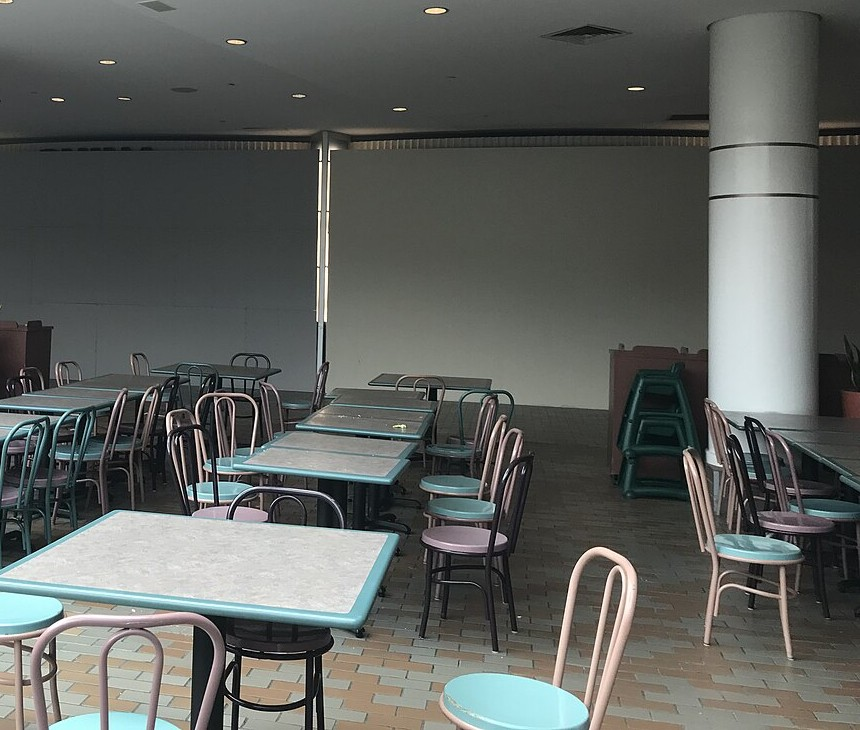
\includegraphics[width=0.45\textwidth]{images/web/empty_food_court_crop.jpg}
\caption[A food court]{A food court, whose tables are shared by everyone who wants to eat at the same time (photo by BornToZucc, cropped, \href{https://creativecommons.org/licenses/by-sa/4.0/}{CC~BY-SA~4.0}, via \href{https://commons.wikimedia.org/}{Wikimedia Commons}).}
\label{fig:intro-foodcourt}
\end{figure}

Several lines of research take this knowledge out of the person. CAROSA gives virtual characters roles, schedules and parameterized actions \citep{allbeck2010carosa}, and functional crowds follow roles and schedules in a building \citep{pelechano2008virtual}. Smart objects contain the information necessary to interact with them \citep{kallmann1999modeling}, characters in The Sims choose objects that advertise what they offer \citep{forbus2001notes}, and the Smart Objects of Unreal Engine let people reserve a slot \citep{epicgames2026smartobjects}. Menge breaks a crowd simulation down into components that can be swapped \citep{curtis2016menge}, and the ODD protocol asks modelers to report the entities and the scheduling of their model \citep{grimm2020odd}.

Our approach builds on these principles, so a person who studies a location should be able to specify the demand with explicit rules and state which resources the environment provides, without having to be a programmer. A new study should also leave the implementation of a person unchanged. Our central idea is that a stated time is a request, that is, a rule that defines when an activity may start, while the simulation decides when it actually starts.

\section{Main Goals}\label{sec:intro-goals}

The aim is to measure how shared resources affect the realized timetable of a place, so that a user can see where and why activities start later than authored. Authored rules, rather than code written for each individual case, give a population of boids purpose, a timetable and a range of activities, and the same system serves every study.

\subsection{Research question}\label{sub:intro-rq}

\begin{quote}
\emph{How can authored rules over capacity-limited stations, followed by a reusable population of boids, show where and why the realized timing of the activities in a place departs from the authored one?}
\end{quote}

The question has a measurement part and an authoring part. The measurement part asks what the recorded runs tell us about waiting, walking and capacity in each place, and the authoring part asks how few rule types and how little scenario code each study needs, as a reusable population keeps the class that represents a person, the movement layer and the resource model the same in every scenario. The scenarios test both parts, because they require routines, shared resources and emergencies to be written in the same way and then measured.

\subsection{Objectives}\label{sub:intro-objectives}

\Cref{chap:problem} sets out the functional requirements R1 to R7, and \cref{chap:conclusions} assesses each of the following objectives against them.

\begin{description}
\item[O1:] A language for purpose and timing, which is an \gls{xml} schedule format that states which person acts, when, with what action and on what target, with explicit rules for deferring, dispatching and dropping rules (R1, R2).
\item[O2:] A movement layer that takes each person to their target by combining navigation mesh path following with boids steering, while the environment, with its walking surfaces, walls, gates and exits, limits movement without being part of the rules (R5).
\item[O3:] Shared resources with a limited capacity, which are stations with places, a first-come, first-served queue and a service time, grouped into areas and used in ordered activities with several stages (R2, R3).
\item[O4:] Reuse across a range of scenarios, with several scenario families in \gls{ue} 5.4 built on a single implementation of a person, to find where reuse breaks down (R4).
\item[O5:] Measurement and a preliminary assessment, which use records of every rule, station visit and trip to show how capacity, travel and population affect the realized timing, and which measure how well the implementation scales on one machine (R6, R7).
\end{description}

\section{Document Structure}\label{sec:intro-structure}

Part~I contains this introduction, \cref{chap:soa} (\nameref{chap:soa}) and \cref{chap:problem} (\nameref{chap:problem}). \Cref{chap:soa} covers boids and steering, agent-based modeling, action selection and crowd models, and the work on purposeful populations, queueing, evacuation and validation. \Cref{chap:problem} describes the behavior we want, gives a high-level overview of our approach without technical detail, sets out the functional requirements R1 to R7 and discusses the difficulties in meeting them.

Part~II, the core of the dissertation, starts with \cref{chap:contribution}, which presents the framework first through the approach built during the pre-dissertation work and then through the architecture of the current pedestrian movement simulator. \Cref{chap:applications} evaluates the system on a daily urban routine, two shopping center layouts, an evacuation and a set of directed-flow corridors, and \cref{chap:conclusions} answers the research question and describes the future work. The appendices contain the per-run result tables (\cref{app:results}) and the build and analysis tooling (\cref{app:tooling}).
